\documentclass[1p]{elsarticle_modified}
%\bibliographystyle{elsarticle-num}

%\usepackage[colorlinks]{hyperref}
%\usepackage{abbrmath_seonhwa} %\Abb, \Ascr, \Acal ,\Abf, \Afrak
\usepackage{amsfonts}
\usepackage{amssymb}
\usepackage{amsmath}
\usepackage{amsthm}
\usepackage{scalefnt}
\usepackage{amsbsy}
\usepackage{kotex}
\usepackage{caption}
\usepackage{subfig}
\usepackage{color}
\usepackage{graphicx}
\usepackage{xcolor} %% white, black, red, green, blue, cyan, magenta, yellow
\usepackage{float}
\usepackage{setspace}
\usepackage{hyperref}

\usepackage{tikz}
\usetikzlibrary{arrows}

\usepackage{multirow}
\usepackage{array} % fixed length table
\usepackage{hhline}

%%%%%%%%%%%%%%%%%%%%%
\makeatletter
\renewcommand*\env@matrix[1][\arraystretch]{%
	\edef\arraystretch{#1}%
	\hskip -\arraycolsep
	\let\@ifnextchar\new@ifnextchar
	\array{*\c@MaxMatrixCols c}}
\makeatother %https://tex.stackexchange.com/questions/14071/how-can-i-increase-the-line-spacing-in-a-matrix
%%%%%%%%%%%%%%%

\usepackage[normalem]{ulem}

\newcommand{\msout}[1]{\ifmmode\text{\sout{\ensuremath{#1}}}\else\sout{#1}\fi}
%SOURCE: \msout is \stkout macro in https://tex.stackexchange.com/questions/20609/strikeout-in-math-mode

\newcommand{\cancel}[1]{
	\ifmmode
	{\color{red}\msout{#1}}
	\else
	{\color{red}\sout{#1}}
	\fi
}

\newcommand{\add}[1]{
	{\color{blue}\uwave{#1}}
}

\newcommand{\replace}[2]{
	\ifmmode
	{\color{red}\msout{#1}}{\color{blue}\uwave{#2}}
	\else
	{\color{red}\sout{#1}}{\color{blue}\uwave{#2}}
	\fi
}

\newcommand{\Sol}{\mathcal{S}} %segment
\newcommand{\D}{D} %diagram
\newcommand{\A}{\mathcal{A}} %arc


%%%%%%%%%%%%%%%%%%%%%%%%%%%%%5 test

\def\sl{\operatorname{\textup{SL}}(2,\Cbb)}
\def\psl{\operatorname{\textup{PSL}}(2,\Cbb)}
\def\quan{\mkern 1mu \triangleright \mkern 1mu}

\theoremstyle{definition}
\newtheorem{thm}{Theorem}[section]
\newtheorem{prop}[thm]{Proposition}
\newtheorem{lem}[thm]{Lemma}
\newtheorem{ques}[thm]{Question}
\newtheorem{cor}[thm]{Corollary}
\newtheorem{defn}[thm]{Definition}
\newtheorem{exam}[thm]{Example}
\newtheorem{rmk}[thm]{Remark}
\newtheorem{alg}[thm]{Algorithm}

\newcommand{\I}{\sqrt{-1}}
\begin{document}

%\begin{frontmatter}
%
%\title{Boundary parabolic representations of knots up to 8 crossings}
%
%%% Group authors per affiliation:
%\author{Yunhi Cho} 
%\address{Department of Mathematics, University of Seoul, Seoul, Korea}
%\ead{yhcho@uos.ac.kr}
%
%
%\author{Seonhwa Kim} %\fnref{s_kim}}
%\address{Center for Geometry and Physics, Institute for Basic Science, Pohang, 37673, Korea}
%\ead{ryeona17@ibs.re.kr}
%
%\author{Hyuk Kim}
%\address{Department of Mathematical Sciences, Seoul National University, Seoul 08826, Korea}
%\ead{hyukkim@snu.ac.kr}
%
%\author{Seokbeom Yoon}
%\address{Department of Mathematical Sciences, Seoul National University, Seoul, 08826,  Korea}
%\ead{sbyoon15@snu.ac.kr}
%
%\begin{abstract}
%We find all boundary parabolic representation of knots up to 8 crossings.
%
%\end{abstract}
%\begin{keyword}
%    \MSC[2010] 57M25 
%\end{keyword}
%
%\end{frontmatter}

%\linenumbers
%\tableofcontents
%
\newcommand\colored[1]{\textcolor{white}{\rule[-0.35ex]{0.8em}{1.4ex}}\kern-0.8em\color{red} #1}%
%\newcommand\colored[1]{\textcolor{white}{ #1}\kern-2.17ex	\textcolor{white}{ #1}\kern-1.81ex	\textcolor{white}{ #1}\kern-2.15ex\color{red}#1	}

{\Large $\underline{12a_{0060}~(K12a_{0060})}$}

\setlength{\tabcolsep}{10pt}
\renewcommand{\arraystretch}{1.6}
\vspace{1cm}\begin{tabular}{m{100pt}>{\centering\arraybackslash}m{274pt}}
\multirow{5}{120pt}{
	\centering
	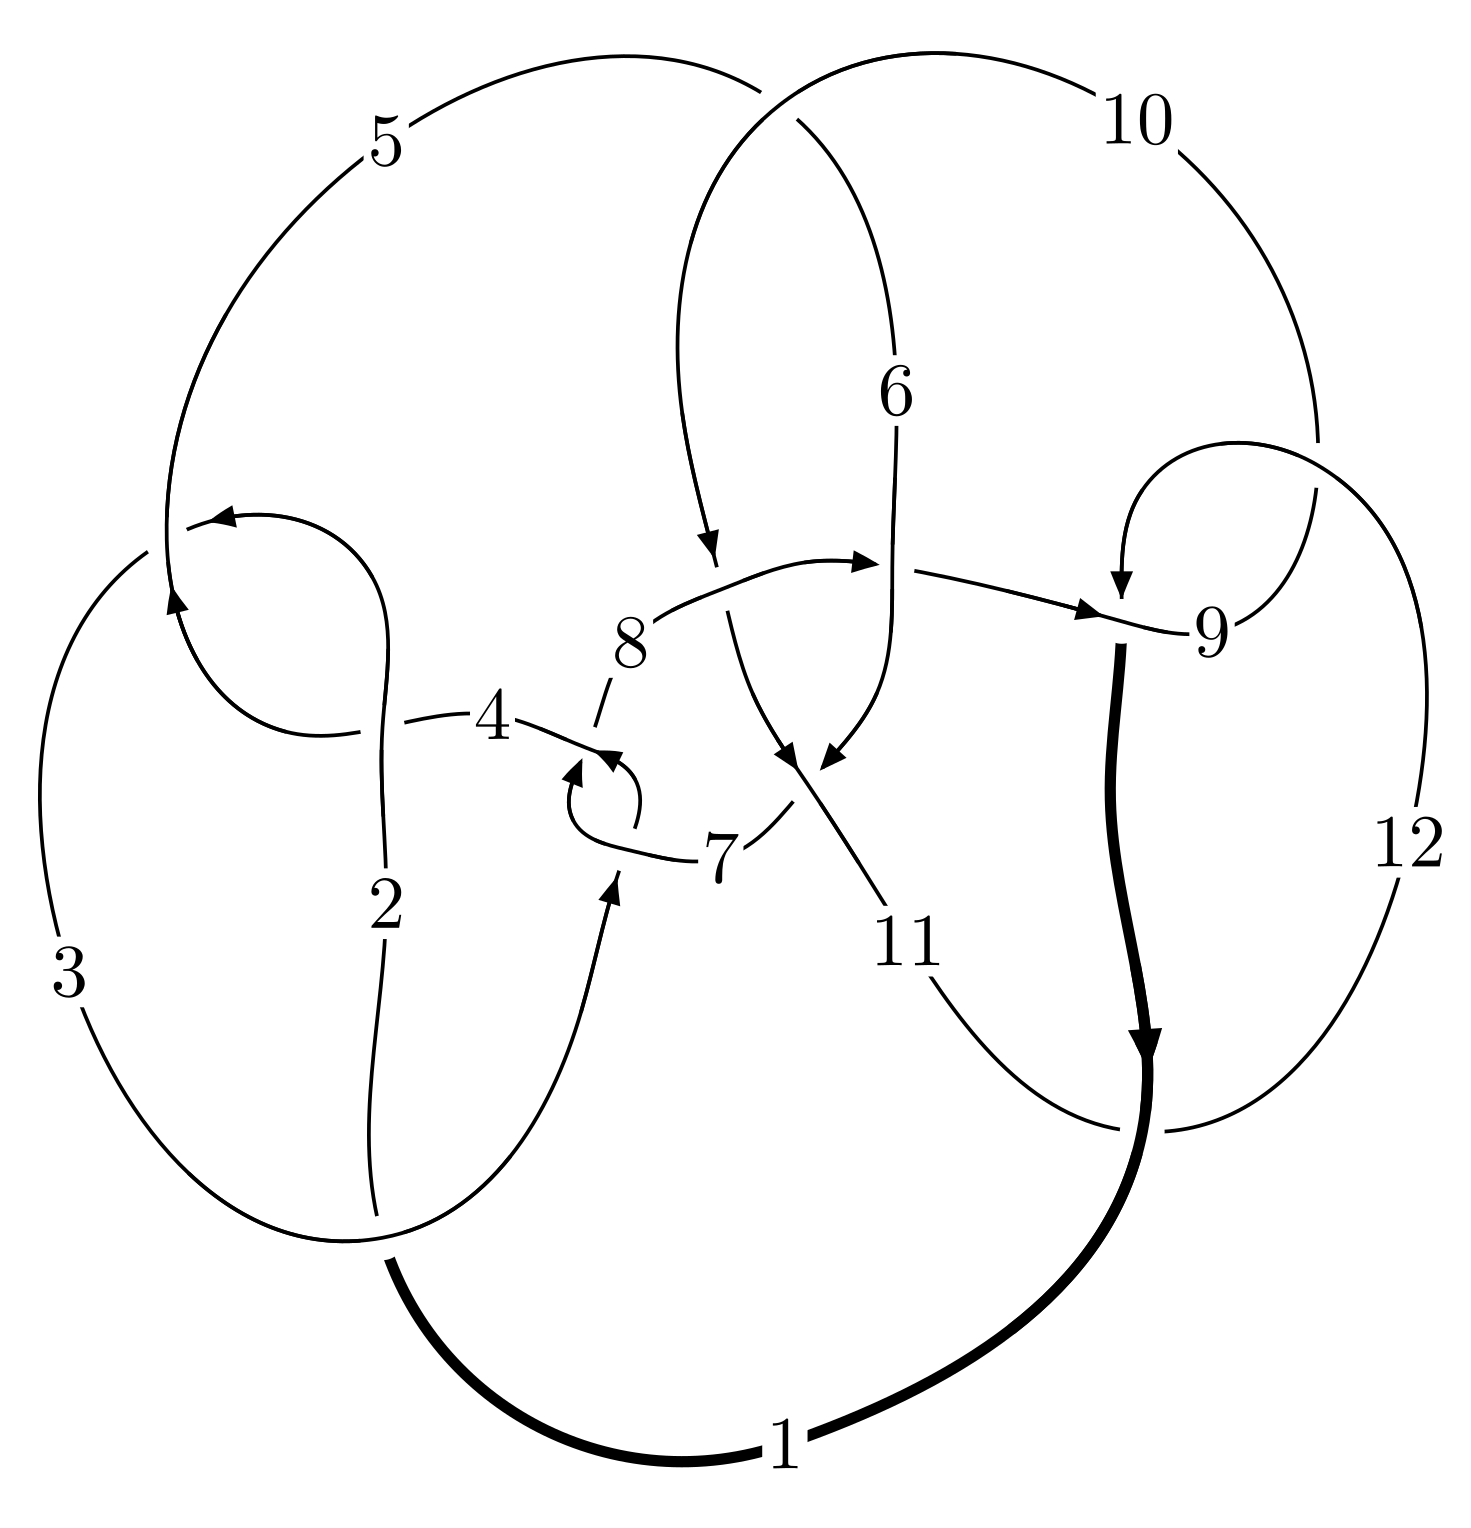
\includegraphics[width=112pt]{../../../GIT/diagram.site/Diagrams/png/861_12a_0060.png}\\
\ \ \ A knot diagram\footnotemark}&
\allowdisplaybreaks
\textbf{Linearized knot diagam} \\
\cline{2-2}
 &
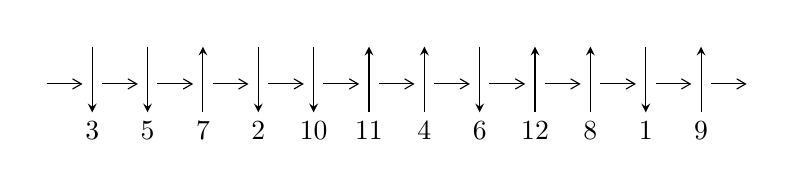
\begin{tikzpicture}[x=20pt, y=17pt]
	% nodes
	\node (C0) at (0, 0) {};
	\node (C1) at (1, 0) {};
	\node (C1U) at (1, +1) {};
	\node (C1D) at (1, -1) {3};

	\node (C2) at (2, 0) {};
	\node (C2U) at (2, +1) {};
	\node (C2D) at (2, -1) {5};

	\node (C3) at (3, 0) {};
	\node (C3U) at (3, +1) {};
	\node (C3D) at (3, -1) {7};

	\node (C4) at (4, 0) {};
	\node (C4U) at (4, +1) {};
	\node (C4D) at (4, -1) {2};

	\node (C5) at (5, 0) {};
	\node (C5U) at (5, +1) {};
	\node (C5D) at (5, -1) {10};

	\node (C6) at (6, 0) {};
	\node (C6U) at (6, +1) {};
	\node (C6D) at (6, -1) {11};

	\node (C7) at (7, 0) {};
	\node (C7U) at (7, +1) {};
	\node (C7D) at (7, -1) {4};

	\node (C8) at (8, 0) {};
	\node (C8U) at (8, +1) {};
	\node (C8D) at (8, -1) {6};

	\node (C9) at (9, 0) {};
	\node (C9U) at (9, +1) {};
	\node (C9D) at (9, -1) {12};

	\node (C10) at (10, 0) {};
	\node (C10U) at (10, +1) {};
	\node (C10D) at (10, -1) {8};

	\node (C11) at (11, 0) {};
	\node (C11U) at (11, +1) {};
	\node (C11D) at (11, -1) {1};

	\node (C12) at (12, 0) {};
	\node (C12U) at (12, +1) {};
	\node (C12D) at (12, -1) {9};
	\node (C13) at (13, 0) {};

	% arrows
	\draw[->,>={angle 60}]
	(C0) edge (C1) (C1) edge (C2) (C2) edge (C3) (C3) edge (C4) (C4) edge (C5) (C5) edge (C6) (C6) edge (C7) (C7) edge (C8) (C8) edge (C9) (C9) edge (C10) (C10) edge (C11) (C11) edge (C12) (C12) edge (C13) ;	\draw[->,>=stealth]
	(C1U) edge (C1D) (C2U) edge (C2D) (C3D) edge (C3U) (C4U) edge (C4D) (C5U) edge (C5D) (C6D) edge (C6U) (C7D) edge (C7U) (C8U) edge (C8D) (C9D) edge (C9U) (C10D) edge (C10U) (C11U) edge (C11D) (C12D) edge (C12U) ;
	\end{tikzpicture} \\
\hhline{~~} \\& 
\textbf{Solving Sequence} \\ \cline{2-2} 
 &
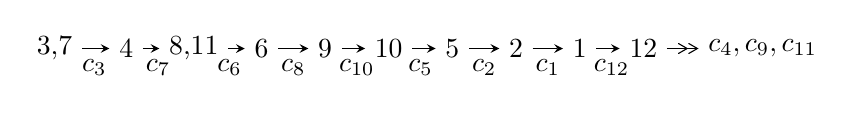
\begin{tikzpicture}[x=23pt, y=7pt]
	% node
	\node (A0) at (-1/8, 0) {3,7};
	\node (A1) at (1, 0) {4};
	\node (A2) at (33/16, 0) {8,11};
	\node (A3) at (25/8, 0) {6};
	\node (A4) at (33/8, 0) {9};
	\node (A5) at (41/8, 0) {10};
	\node (A6) at (49/8, 0) {5};
	\node (A7) at (57/8, 0) {2};
	\node (A8) at (65/8, 0) {1};
	\node (A9) at (73/8, 0) {12};
	\node (C1) at (1/2, -1) {$c_{3}$};
	\node (C2) at (3/2, -1) {$c_{7}$};
	\node (C3) at (21/8, -1) {$c_{6}$};
	\node (C4) at (29/8, -1) {$c_{8}$};
	\node (C5) at (37/8, -1) {$c_{10}$};
	\node (C6) at (45/8, -1) {$c_{5}$};
	\node (C7) at (53/8, -1) {$c_{2}$};
	\node (C8) at (61/8, -1) {$c_{1}$};
	\node (C9) at (69/8, -1) {$c_{12}$};
	\node (A10) at (11, 0) {$c_{4},c_{9},c_{11}$};

	% edge
	\draw[->,>=stealth]	
	(A0) edge (A1) (A1) edge (A2) (A2) edge (A3) (A3) edge (A4) (A4) edge (A5) (A5) edge (A6) (A6) edge (A7) (A7) edge (A8) (A8) edge (A9) ;
	\draw[->>,>={angle 60}]	
	(A9) edge (A10);
\end{tikzpicture} \\ 

\end{tabular} \\

\footnotetext{
The image of knot diagram is generated by the software ``\textbf{Draw programme}" developed by Andrew Bartholomew(\url{http://www.layer8.co.uk/maths/draw/index.htm\#Running-draw}), where we modified some parts for our purpose(\url{https://github.com/CATsTAILs/LinksPainter}).
}\phantom \\ \newline 
\centering \textbf{Ideals for irreducible components\footnotemark of $X_{\text{par}}$} 
 
\begin{align*}
I^u_{1}&=\langle 
2.82224\times10^{566} u^{139}+1.76219\times10^{566} u^{138}+\cdots+1.62257\times10^{567} b+7.22892\times10^{569},\\
\phantom{I^u_{1}}&\phantom{= \langle  }1.07751\times10^{567} u^{139}+6.57014\times10^{566} u^{138}+\cdots+1.62257\times10^{567} a+2.82386\times10^{570},\\
\phantom{I^u_{1}}&\phantom{= \langle  }u^{140}+u^{139}+\cdots+8192 u+1024\rangle \\
\\
I^v_{1}&=\langle 
a,\;4 v^3-6 v^2+b+25 v-8,\;v^4-2 v^3+7 v^2-5 v+1\rangle \\
I^v_{2}&=\langle 
a,\;50 v^5+61 v^4+196 v^3+119 v^2+67 b+390 v+59,\;v^6+v^5+4 v^4+2 v^3+8 v^2+1\rangle \\
\end{align*}
\raggedright * 3 irreducible components of $\dim_{\mathbb{C}}=0$, with total 150 representations.\\
\footnotetext{All coefficients of polynomials are rational numbers. But the coefficients are sometimes approximated in decimal forms when there is not enough margin.}
\newpage
\renewcommand{\arraystretch}{1}
\centering \section*{I. $I^u_{1}= \langle 2.82\times10^{566} u^{139}+1.76\times10^{566} u^{138}+\cdots+1.62\times10^{567} b+7.23\times10^{569},\;1.08\times10^{567} u^{139}+6.57\times10^{566} u^{138}+\cdots+1.62\times10^{567} a+2.82\times10^{570},\;u^{140}+u^{139}+\cdots+8192 u+1024 \rangle$}
\flushleft \textbf{(i) Arc colorings}\\
\begin{tabular}{m{7pt} m{180pt} m{7pt} m{180pt} }
\flushright $a_{3}=$&$\begin{pmatrix}1\\0\end{pmatrix}$ \\
\flushright $a_{7}=$&$\begin{pmatrix}0\\u\end{pmatrix}$ \\
\flushright $a_{4}=$&$\begin{pmatrix}1\\- u^2\end{pmatrix}$ \\
\flushright $a_{8}=$&$\begin{pmatrix}u\\- u^3+u\end{pmatrix}$ \\
\flushright $a_{11}=$&$\begin{pmatrix}-0.664076 u^{139}-0.404921 u^{138}+\cdots-9478.56 u-1740.36\\-0.173936 u^{139}-0.108605 u^{138}+\cdots-2458.67 u-445.522\end{pmatrix}$ \\
\flushright $a_{6}=$&$\begin{pmatrix}-0.599073 u^{139}-0.372142 u^{138}+\cdots-8619.84 u-1591.58\\-0.0565797 u^{139}-0.0188547 u^{138}+\cdots-546.416 u-86.8817\end{pmatrix}$ \\
\flushright $a_{9}=$&$\begin{pmatrix}0.235557 u^{139}+0.145522 u^{138}+\cdots+3360.46 u+608.447\\0.204961 u^{139}+0.119227 u^{138}+\cdots+2804.73 u+505.380\end{pmatrix}$ \\
\flushright $a_{10}=$&$\begin{pmatrix}-0.729961 u^{139}-0.437305 u^{138}+\cdots-10338.5 u-1897.61\\-0.219084 u^{139}-0.134689 u^{138}+\cdots-3111.68 u-568.463\end{pmatrix}$ \\
\flushright $a_{5}=$&$\begin{pmatrix}-0.00229243 u^{139}-0.00688234 u^{138}+\cdots-119.334 u-22.0563\\0.0224336 u^{139}+0.00780471 u^{138}+\cdots+256.104 u+43.2884\end{pmatrix}$ \\
\flushright $a_{2}=$&$\begin{pmatrix}-0.00229243 u^{139}-0.00688234 u^{138}+\cdots-119.334 u-22.0563\\-0.0265260 u^{139}-0.0110130 u^{138}+\cdots-296.052 u-47.9885\end{pmatrix}$ \\
\flushright $a_{1}=$&$\begin{pmatrix}-0.0288184 u^{139}-0.0178953 u^{138}+\cdots-415.385 u-70.0448\\-0.0265260 u^{139}-0.0110130 u^{138}+\cdots-296.052 u-47.9885\end{pmatrix}$ \\
\flushright $a_{12}=$&$\begin{pmatrix}-0.459995 u^{139}-0.286124 u^{138}+\cdots-6634.61 u-1213.55\\-0.193301 u^{139}-0.112910 u^{138}+\cdots-2650.68 u-476.747\end{pmatrix}$\\&\end{tabular}
\flushleft \textbf{(ii) Obstruction class $= -1$}\\~\\
\flushleft \textbf{(iii) Cusp Shapes $= 1.69069 u^{139}+1.00549 u^{138}+\cdots+23555.4 u+4256.25$}\\~\\
\newpage\renewcommand{\arraystretch}{1}
\flushleft \textbf{(iv) u-Polynomials at the component}\newline \\
\begin{tabular}{m{50pt}|m{274pt}}
Crossings & \hspace{64pt}u-Polynomials at each crossing \\
\hline $$\begin{aligned}c_{1}\end{aligned}$$&$\begin{aligned}
&u^{140}+69 u^{139}+\cdots+221 u+1
\end{aligned}$\\
\hline $$\begin{aligned}c_{2},c_{4}\end{aligned}$$&$\begin{aligned}
&u^{140}-11 u^{139}+\cdots-5 u+1
\end{aligned}$\\
\hline $$\begin{aligned}c_{3},c_{7}\end{aligned}$$&$\begin{aligned}
&u^{140}- u^{139}+\cdots-8192 u+1024
\end{aligned}$\\
\hline $$\begin{aligned}c_{5}\end{aligned}$$&$\begin{aligned}
&u^{140}+2 u^{139}+\cdots-10624 u+1216
\end{aligned}$\\
\hline $$\begin{aligned}c_{6}\end{aligned}$$&$\begin{aligned}
&u^{140}-2 u^{139}+\cdots-24012 u+5887
\end{aligned}$\\
\hline $$\begin{aligned}c_{8}\end{aligned}$$&$\begin{aligned}
&u^{140}-10 u^{139}+\cdots-2 u+1
\end{aligned}$\\
\hline $$\begin{aligned}c_{9},c_{12}\end{aligned}$$&$\begin{aligned}
&u^{140}+2 u^{139}+\cdots+14 u+1
\end{aligned}$\\
\hline $$\begin{aligned}c_{10}\end{aligned}$$&$\begin{aligned}
&u^{140}+14 u^{139}+\cdots+2 u+1
\end{aligned}$\\
\hline $$\begin{aligned}c_{11}\end{aligned}$$&$\begin{aligned}
&u^{140}+58 u^{139}+\cdots+14 u+1
\end{aligned}$\\
\hline
\end{tabular}\\~\\
\newpage\renewcommand{\arraystretch}{1}
\flushleft \textbf{(v) Riley Polynomials at the component}\newline \\
\begin{tabular}{m{50pt}|m{274pt}}
Crossings & \hspace{64pt}Riley Polynomials at each crossing \\
\hline $$\begin{aligned}c_{1}\end{aligned}$$&$\begin{aligned}
&y^{140}+15 y^{139}+\cdots-2817 y+1
\end{aligned}$\\
\hline $$\begin{aligned}c_{2},c_{4}\end{aligned}$$&$\begin{aligned}
&y^{140}-69 y^{139}+\cdots-221 y+1
\end{aligned}$\\
\hline $$\begin{aligned}c_{3},c_{7}\end{aligned}$$&$\begin{aligned}
&y^{140}-63 y^{139}+\cdots-25690112 y+1048576
\end{aligned}$\\
\hline $$\begin{aligned}c_{5}\end{aligned}$$&$\begin{aligned}
&y^{140}+150 y^{139}+\cdots+35716096 y+1478656
\end{aligned}$\\
\hline $$\begin{aligned}c_{6}\end{aligned}$$&$\begin{aligned}
&y^{140}+142 y^{139}+\cdots+261556046 y+34656769
\end{aligned}$\\
\hline $$\begin{aligned}c_{8}\end{aligned}$$&$\begin{aligned}
&y^{140}+14 y^{139}+\cdots+10 y+1
\end{aligned}$\\
\hline $$\begin{aligned}c_{9},c_{12}\end{aligned}$$&$\begin{aligned}
&y^{140}+58 y^{139}+\cdots+14 y+1
\end{aligned}$\\
\hline $$\begin{aligned}c_{10}\end{aligned}$$&$\begin{aligned}
&y^{140}+10 y^{139}+\cdots+14 y+1
\end{aligned}$\\
\hline $$\begin{aligned}c_{11}\end{aligned}$$&$\begin{aligned}
&y^{140}+50 y^{139}+\cdots-2010 y+1
\end{aligned}$\\
\hline
\end{tabular}\\~\\
\newpage\flushleft \textbf{(vi) Complex Volumes and Cusp Shapes}
$$\begin{array}{c|c|c}  
\text{Solutions to }I^u_{1}& \I (\text{vol} + \sqrt{-1}CS) & \text{Cusp shape}\\
 \hline 
\begin{aligned}
u &= \phantom{-}1.000760 + 0.012534 I \\
a &= -0.306225 + 0.320226 I \\
b &= -1.40232 + 0.29598 I\end{aligned}
 & \phantom{-}0.24476 - 4.35802 I & \phantom{-0.000000 } 0 \\ \hline\begin{aligned}
u &= \phantom{-}1.000760 - 0.012534 I \\
a &= -0.306225 - 0.320226 I \\
b &= -1.40232 - 0.29598 I\end{aligned}
 & \phantom{-}0.24476 + 4.35802 I & \phantom{-0.000000 } 0 \\ \hline\begin{aligned}
u &= -0.836596 + 0.555007 I \\
a &= \phantom{-}1.006110 - 0.475231 I \\
b &= \phantom{-}2.42428 + 0.23434 I\end{aligned}
 & -6.69476 - 2.77249 I & \phantom{-0.000000 } 0 \\ \hline\begin{aligned}
u &= -0.836596 - 0.555007 I \\
a &= \phantom{-}1.006110 + 0.475231 I \\
b &= \phantom{-}2.42428 - 0.23434 I\end{aligned}
 & -6.69476 + 2.77249 I & \phantom{-0.000000 } 0 \\ \hline\begin{aligned}
u &= -0.421062 + 0.872083 I \\
a &= \phantom{-}0.206555 - 0.622102 I \\
b &= \phantom{-}2.25386 - 0.11399 I\end{aligned}
 & -1.36351 + 5.67921 I & \phantom{-0.000000 } 0 \\ \hline\begin{aligned}
u &= -0.421062 - 0.872083 I \\
a &= \phantom{-}0.206555 + 0.622102 I \\
b &= \phantom{-}2.25386 + 0.11399 I\end{aligned}
 & -1.36351 - 5.67921 I & \phantom{-0.000000 } 0 \\ \hline\begin{aligned}
u &= \phantom{-}0.189163 + 1.024150 I \\
a &= \phantom{-}0.531321 + 1.025970 I \\
b &= \phantom{-}0.786265 + 0.856529 I\end{aligned}
 & \phantom{-}1.66936 - 3.03245 I & \phantom{-0.000000 } 0 \\ \hline\begin{aligned}
u &= \phantom{-}0.189163 - 1.024150 I \\
a &= \phantom{-}0.531321 - 1.025970 I \\
b &= \phantom{-}0.786265 - 0.856529 I\end{aligned}
 & \phantom{-}1.66936 + 3.03245 I & \phantom{-0.000000 } 0 \\ \hline\begin{aligned}
u &= -0.797095 + 0.513895 I \\
a &= \phantom{-}0.215390 - 1.374710 I \\
b &= \phantom{-}0.997714 + 0.916821 I\end{aligned}
 & -6.83212 - 1.55059 I & \phantom{-0.000000 } 0 \\ \hline\begin{aligned}
u &= -0.797095 - 0.513895 I \\
a &= \phantom{-}0.215390 + 1.374710 I \\
b &= \phantom{-}0.997714 - 0.916821 I\end{aligned}
 & -6.83212 + 1.55059 I & \phantom{-0.000000 } 0\\
 \hline 
 \end{array}$$\newpage$$\begin{array}{c|c|c}  
\text{Solutions to }I^u_{1}& \I (\text{vol} + \sqrt{-1}CS) & \text{Cusp shape}\\
 \hline 
\begin{aligned}
u &= -0.682457 + 0.821355 I \\
a &= \phantom{-}0.276201 - 0.036517 I \\
b &= -0.249515 + 0.258948 I\end{aligned}
 & \phantom{-}0.47320 - 1.54565 I & \phantom{-0.000000 } 0 \\ \hline\begin{aligned}
u &= -0.682457 - 0.821355 I \\
a &= \phantom{-}0.276201 + 0.036517 I \\
b &= -0.249515 - 0.258948 I\end{aligned}
 & \phantom{-}0.47320 + 1.54565 I & \phantom{-0.000000 } 0 \\ \hline\begin{aligned}
u &= -0.992021 + 0.397301 I \\
a &= -1.195460 + 0.435861 I \\
b &= -1.70698 - 0.28925 I\end{aligned}
 & -0.77366 - 5.05718 I & \phantom{-0.000000 } 0 \\ \hline\begin{aligned}
u &= -0.992021 - 0.397301 I \\
a &= -1.195460 - 0.435861 I \\
b &= -1.70698 + 0.28925 I\end{aligned}
 & -0.77366 + 5.05718 I & \phantom{-0.000000 } 0 \\ \hline\begin{aligned}
u &= \phantom{-}0.357797 + 0.844946 I \\
a &= -0.364638 - 0.836942 I \\
b &= -0.852570 - 0.691242 I\end{aligned}
 & -1.82288 - 1.42035 I & \phantom{-0.000000 } 0 \\ \hline\begin{aligned}
u &= \phantom{-}0.357797 - 0.844946 I \\
a &= -0.364638 + 0.836942 I \\
b &= -0.852570 + 0.691242 I\end{aligned}
 & -1.82288 + 1.42035 I & \phantom{-0.000000 } 0 \\ \hline\begin{aligned}
u &= -1.002640 + 0.433199 I \\
a &= \phantom{-}0.191557 - 0.047478 I \\
b &= \phantom{-}1.55074 + 0.59070 I\end{aligned}
 & -0.811795 + 0.033701 I & \phantom{-0.000000 } 0 \\ \hline\begin{aligned}
u &= -1.002640 - 0.433199 I \\
a &= \phantom{-}0.191557 + 0.047478 I \\
b &= \phantom{-}1.55074 - 0.59070 I\end{aligned}
 & -0.811795 - 0.033701 I & \phantom{-0.000000 } 0 \\ \hline\begin{aligned}
u &= -0.575665 + 0.936495 I \\
a &= \phantom{-}0.395098 - 0.932422 I \\
b &= \phantom{-}1.249570 + 0.340721 I\end{aligned}
 & -6.19030 + 5.36695 I & \phantom{-0.000000 } 0 \\ \hline\begin{aligned}
u &= -0.575665 - 0.936495 I \\
a &= \phantom{-}0.395098 + 0.932422 I \\
b &= \phantom{-}1.249570 - 0.340721 I\end{aligned}
 & -6.19030 - 5.36695 I & \phantom{-0.000000 } 0\\
 \hline 
 \end{array}$$\newpage$$\begin{array}{c|c|c}  
\text{Solutions to }I^u_{1}& \I (\text{vol} + \sqrt{-1}CS) & \text{Cusp shape}\\
 \hline 
\begin{aligned}
u &= -1.068570 + 0.259692 I \\
a &= \phantom{-}0.56267 - 2.76229 I \\
b &= \phantom{-}1.49656 + 0.99735 I\end{aligned}
 & \phantom{-}2.38264 + 1.08657 I & \phantom{-0.000000 } 0 \\ \hline\begin{aligned}
u &= -1.068570 - 0.259692 I \\
a &= \phantom{-}0.56267 + 2.76229 I \\
b &= \phantom{-}1.49656 - 0.99735 I\end{aligned}
 & \phantom{-}2.38264 - 1.08657 I & \phantom{-0.000000 } 0 \\ \hline\begin{aligned}
u &= \phantom{-}0.798347 + 0.415330 I \\
a &= -0.679635 - 1.152670 I \\
b &= -0.486148 + 0.821596 I\end{aligned}
 & -2.17880 + 4.32767 I & \phantom{-0.000000 } 0 \\ \hline\begin{aligned}
u &= \phantom{-}0.798347 - 0.415330 I \\
a &= -0.679635 + 1.152670 I \\
b &= -0.486148 - 0.821596 I\end{aligned}
 & -2.17880 - 4.32767 I & \phantom{-0.000000 } 0 \\ \hline\begin{aligned}
u &= -0.299839 + 0.848133 I \\
a &= \phantom{-}0.150645 + 0.978113 I \\
b &= \phantom{-}0.744768 + 0.363732 I\end{aligned}
 & \phantom{-}0.79500 + 3.33230 I & \phantom{-0.000000 } 0 \\ \hline\begin{aligned}
u &= -0.299839 - 0.848133 I \\
a &= \phantom{-}0.150645 - 0.978113 I \\
b &= \phantom{-}0.744768 - 0.363732 I\end{aligned}
 & \phantom{-}0.79500 - 3.33230 I & \phantom{-0.000000 } 0 \\ \hline\begin{aligned}
u &= -1.047890 + 0.343169 I \\
a &= -0.88012 + 3.01481 I \\
b &= -2.29815 - 1.00177 I\end{aligned}
 & \phantom{-}2.07851 - 3.32587 I & \phantom{-0.000000 } 0 \\ \hline\begin{aligned}
u &= -1.047890 - 0.343169 I \\
a &= -0.88012 - 3.01481 I \\
b &= -2.29815 + 1.00177 I\end{aligned}
 & \phantom{-}2.07851 + 3.32587 I & \phantom{-0.000000 } 0 \\ \hline\begin{aligned}
u &= -0.866740 + 0.208182 I \\
a &= -0.58859 + 1.77401 I \\
b &= -1.389370 - 0.112852 I\end{aligned}
 & \phantom{-}1.10254 + 1.14634 I & \phantom{-0.000000 } 0 \\ \hline\begin{aligned}
u &= -0.866740 - 0.208182 I \\
a &= -0.58859 - 1.77401 I \\
b &= -1.389370 + 0.112852 I\end{aligned}
 & \phantom{-}1.10254 - 1.14634 I & \phantom{-0.000000 } 0\\
 \hline 
 \end{array}$$\newpage$$\begin{array}{c|c|c}  
\text{Solutions to }I^u_{1}& \I (\text{vol} + \sqrt{-1}CS) & \text{Cusp shape}\\
 \hline 
\begin{aligned}
u &= -0.650609 + 0.588985 I \\
a &= \phantom{-}0.354024 - 0.405783 I \\
b &= -0.1023010 + 0.0046218 I\end{aligned}
 & \phantom{-}0.44265 - 1.56279 I & \phantom{-0.000000 } 0 \\ \hline\begin{aligned}
u &= -0.650609 - 0.588985 I \\
a &= \phantom{-}0.354024 + 0.405783 I \\
b &= -0.1023010 - 0.0046218 I\end{aligned}
 & \phantom{-}0.44265 + 1.56279 I & \phantom{-0.000000 } 0 \\ \hline\begin{aligned}
u &= \phantom{-}0.661212 + 0.572663 I \\
a &= \phantom{-}0.921225 + 0.672046 I \\
b &= \phantom{-}0.279894 - 0.814023 I\end{aligned}
 & -4.97493 + 8.44093 I & \phantom{-0.000000 } 0 \\ \hline\begin{aligned}
u &= \phantom{-}0.661212 - 0.572663 I \\
a &= \phantom{-}0.921225 - 0.672046 I \\
b &= \phantom{-}0.279894 + 0.814023 I\end{aligned}
 & -4.97493 - 8.44093 I & \phantom{-0.000000 } 0 \\ \hline\begin{aligned}
u &= \phantom{-}1.114470 + 0.173765 I \\
a &= -0.712327 + 0.632019 I \\
b &= -0.397554 - 1.170360 I\end{aligned}
 & \phantom{-}3.91294 - 3.33139 I & \phantom{-0.000000 } 0 \\ \hline\begin{aligned}
u &= \phantom{-}1.114470 - 0.173765 I \\
a &= -0.712327 - 0.632019 I \\
b &= -0.397554 + 1.170360 I\end{aligned}
 & \phantom{-}3.91294 + 3.33139 I & \phantom{-0.000000 } 0 \\ \hline\begin{aligned}
u &= \phantom{-}0.286617 + 1.097040 I \\
a &= -0.578658 - 1.101670 I \\
b &= -1.32911 - 0.99991 I\end{aligned}
 & -0.05649 - 8.46319 I & \phantom{-0.000000 } 0 \\ \hline\begin{aligned}
u &= \phantom{-}0.286617 - 1.097040 I \\
a &= -0.578658 + 1.101670 I \\
b &= -1.32911 + 0.99991 I\end{aligned}
 & -0.05649 + 8.46319 I & \phantom{-0.000000 } 0 \\ \hline\begin{aligned}
u &= \phantom{-}0.427712 + 0.750160 I \\
a &= -0.704498 - 1.018660 I \\
b &= -1.081150 + 0.346220 I\end{aligned}
 & -3.82479 - 1.32683 I & \phantom{-0.000000 } 0 \\ \hline\begin{aligned}
u &= \phantom{-}0.427712 - 0.750160 I \\
a &= -0.704498 + 1.018660 I \\
b &= -1.081150 - 0.346220 I\end{aligned}
 & -3.82479 + 1.32683 I & \phantom{-0.000000 } 0\\
 \hline 
 \end{array}$$\newpage$$\begin{array}{c|c|c}  
\text{Solutions to }I^u_{1}& \I (\text{vol} + \sqrt{-1}CS) & \text{Cusp shape}\\
 \hline 
\begin{aligned}
u &= \phantom{-}0.435388 + 0.743385 I \\
a &= \phantom{-}3.24340 + 2.10472 I \\
b &= \phantom{-}6.13829 + 0.59251 I\end{aligned}
 & -1.93443 - 3.19824 I & \phantom{-0.000000 } 0 \\ \hline\begin{aligned}
u &= \phantom{-}0.435388 - 0.743385 I \\
a &= \phantom{-}3.24340 - 2.10472 I \\
b &= \phantom{-}6.13829 - 0.59251 I\end{aligned}
 & -1.93443 + 3.19824 I & \phantom{-0.000000 } 0 \\ \hline\begin{aligned}
u &= \phantom{-}1.018440 + 0.525386 I \\
a &= \phantom{-}1.32268 + 1.57773 I \\
b &= \phantom{-}2.52977 - 1.33691 I\end{aligned}
 & -0.66742 + 3.20117 I & \phantom{-0.000000 } 0 \\ \hline\begin{aligned}
u &= \phantom{-}1.018440 - 0.525386 I \\
a &= \phantom{-}1.32268 - 1.57773 I \\
b &= \phantom{-}2.52977 + 1.33691 I\end{aligned}
 & -0.66742 - 3.20117 I & \phantom{-0.000000 } 0 \\ \hline\begin{aligned}
u &= -0.213477 + 0.816553 I \\
a &= \phantom{-}0.173255 + 0.561079 I \\
b &= -1.064580 - 0.152324 I\end{aligned}
 & \phantom{-}1.043390 + 0.077155 I & \phantom{-0.000000 } 0 \\ \hline\begin{aligned}
u &= -0.213477 - 0.816553 I \\
a &= \phantom{-}0.173255 - 0.561079 I \\
b &= -1.064580 + 0.152324 I\end{aligned}
 & \phantom{-}1.043390 - 0.077155 I & \phantom{-0.000000 } 0 \\ \hline\begin{aligned}
u &= -1.062380 + 0.456587 I \\
a &= \phantom{-}1.228930 - 0.504376 I \\
b &= \phantom{-}1.68579 + 0.64955 I\end{aligned}
 & -2.70777 - 10.63070 I & \phantom{-0.000000 } 0 \\ \hline\begin{aligned}
u &= -1.062380 - 0.456587 I \\
a &= \phantom{-}1.228930 + 0.504376 I \\
b &= \phantom{-}1.68579 - 0.64955 I\end{aligned}
 & -2.70777 + 10.63070 I & \phantom{-0.000000 } 0 \\ \hline\begin{aligned}
u &= -1.121250 + 0.296975 I \\
a &= \phantom{-}1.149810 - 0.253365 I \\
b &= \phantom{-}0.471235 + 0.734948 I\end{aligned}
 & \phantom{-}2.53463 - 1.34948 I & \phantom{-0.000000 } 0 \\ \hline\begin{aligned}
u &= -1.121250 - 0.296975 I \\
a &= \phantom{-}1.149810 + 0.253365 I \\
b &= \phantom{-}0.471235 - 0.734948 I\end{aligned}
 & \phantom{-}2.53463 + 1.34948 I & \phantom{-0.000000 } 0\\
 \hline 
 \end{array}$$\newpage$$\begin{array}{c|c|c}  
\text{Solutions to }I^u_{1}& \I (\text{vol} + \sqrt{-1}CS) & \text{Cusp shape}\\
 \hline 
\begin{aligned}
u &= \phantom{-}1.150790 + 0.258089 I \\
a &= \phantom{-}0.554520 + 0.096579 I \\
b &= \phantom{-}1.03502 - 1.39865 I\end{aligned}
 & \phantom{-}5.51111 - 0.29685 I & \phantom{-0.000000 } 0 \\ \hline\begin{aligned}
u &= \phantom{-}1.150790 - 0.258089 I \\
a &= \phantom{-}0.554520 - 0.096579 I \\
b &= \phantom{-}1.03502 + 1.39865 I\end{aligned}
 & \phantom{-}5.51111 + 0.29685 I & \phantom{-0.000000 } 0 \\ \hline\begin{aligned}
u &= \phantom{-}1.112440 + 0.403471 I \\
a &= -0.580315 - 0.363099 I \\
b &= -0.98833 + 1.94189 I\end{aligned}
 & \phantom{-}2.99181 + 5.97516 I & \phantom{-0.000000 } 0 \\ \hline\begin{aligned}
u &= \phantom{-}1.112440 - 0.403471 I \\
a &= -0.580315 + 0.363099 I \\
b &= -0.98833 - 1.94189 I\end{aligned}
 & \phantom{-}2.99181 - 5.97516 I & \phantom{-0.000000 } 0 \\ \hline\begin{aligned}
u &= \phantom{-}1.145340 + 0.322180 I \\
a &= \phantom{-}0.799528 - 0.226577 I \\
b &= \phantom{-}0.887250 + 0.424942 I\end{aligned}
 & \phantom{-}5.25058 + 3.26329 I & \phantom{-0.000000 } 0 \\ \hline\begin{aligned}
u &= \phantom{-}1.145340 - 0.322180 I \\
a &= \phantom{-}0.799528 + 0.226577 I \\
b &= \phantom{-}0.887250 - 0.424942 I\end{aligned}
 & \phantom{-}5.25058 - 3.26329 I & \phantom{-0.000000 } 0 \\ \hline\begin{aligned}
u &= -0.502968 + 1.083090 I \\
a &= -0.332049 + 1.189060 I \\
b &= -1.45374 + 0.78148 I\end{aligned}
 & \phantom{-}0.11630 + 7.78284 I & \phantom{-0.000000 } 0 \\ \hline\begin{aligned}
u &= -0.502968 - 1.083090 I \\
a &= -0.332049 - 1.189060 I \\
b &= -1.45374 - 0.78148 I\end{aligned}
 & \phantom{-}0.11630 - 7.78284 I & \phantom{-0.000000 } 0 \\ \hline\begin{aligned}
u &= \phantom{-}0.651482 + 0.461118 I \\
a &= -0.659951 - 0.466565 I \\
b &= -1.082100 - 0.435986 I\end{aligned}
 & -2.43454 - 0.65211 I & \phantom{-0.000000 } 0 \\ \hline\begin{aligned}
u &= \phantom{-}0.651482 - 0.461118 I \\
a &= -0.659951 + 0.466565 I \\
b &= -1.082100 + 0.435986 I\end{aligned}
 & -2.43454 + 0.65211 I & \phantom{-0.000000 } 0\\
 \hline 
 \end{array}$$\newpage$$\begin{array}{c|c|c}  
\text{Solutions to }I^u_{1}& \I (\text{vol} + \sqrt{-1}CS) & \text{Cusp shape}\\
 \hline 
\begin{aligned}
u &= \phantom{-}1.073680 + 0.545137 I \\
a &= -0.835240 - 0.325325 I \\
b &= -1.83968 + 0.59135 I\end{aligned}
 & -1.88588 + 6.17613 I & \phantom{-0.000000 } 0 \\ \hline\begin{aligned}
u &= \phantom{-}1.073680 - 0.545137 I \\
a &= -0.835240 + 0.325325 I \\
b &= -1.83968 - 0.59135 I\end{aligned}
 & -1.88588 - 6.17613 I & \phantom{-0.000000 } 0 \\ \hline\begin{aligned}
u &= \phantom{-}0.329298 + 0.722391 I \\
a &= -2.66753 - 1.82474 I \\
b &= -5.11037 - 1.17767 I\end{aligned}
 & -1.66193 + 0.85450 I & \phantom{-0.000000 } 0 \\ \hline\begin{aligned}
u &= \phantom{-}0.329298 - 0.722391 I \\
a &= -2.66753 + 1.82474 I \\
b &= -5.11037 + 1.17767 I\end{aligned}
 & -1.66193 - 0.85450 I & \phantom{-0.000000 } 0 \\ \hline\begin{aligned}
u &= -1.116010 + 0.465367 I \\
a &= \phantom{-}0.632935 + 0.748697 I \\
b &= \phantom{-}0.011210 - 0.645952 I\end{aligned}
 & \phantom{-}2.54912 - 1.64137 I & \phantom{-0.000000 } 0 \\ \hline\begin{aligned}
u &= -1.116010 - 0.465367 I \\
a &= \phantom{-}0.632935 - 0.748697 I \\
b &= \phantom{-}0.011210 + 0.645952 I\end{aligned}
 & \phantom{-}2.54912 + 1.64137 I & \phantom{-0.000000 } 0 \\ \hline\begin{aligned}
u &= \phantom{-}0.182675 + 1.199720 I \\
a &= -0.515031 - 0.404484 I \\
b &= -1.067950 - 0.429971 I\end{aligned}
 & -1.95759 - 0.96618 I & \phantom{-0.000000 } 0 \\ \hline\begin{aligned}
u &= \phantom{-}0.182675 - 1.199720 I \\
a &= -0.515031 + 0.404484 I \\
b &= -1.067950 + 0.429971 I\end{aligned}
 & -1.95759 + 0.96618 I & \phantom{-0.000000 } 0 \\ \hline\begin{aligned}
u &= -0.704978 + 0.343098 I \\
a &= \phantom{-}0.02805 + 1.80042 I \\
b &= -0.796426 - 0.591122 I\end{aligned}
 & -1.78233 + 1.83282 I & \phantom{-0.000000 } 0 \\ \hline\begin{aligned}
u &= -0.704978 - 0.343098 I \\
a &= \phantom{-}0.02805 - 1.80042 I \\
b &= -0.796426 + 0.591122 I\end{aligned}
 & -1.78233 - 1.83282 I & \phantom{-0.000000 } 0\\
 \hline 
 \end{array}$$\newpage$$\begin{array}{c|c|c}  
\text{Solutions to }I^u_{1}& \I (\text{vol} + \sqrt{-1}CS) & \text{Cusp shape}\\
 \hline 
\begin{aligned}
u &= \phantom{-}0.505815 + 0.581629 I \\
a &= \phantom{-}3.01807 + 1.77462 I \\
b &= \phantom{-}4.63447 - 0.19221 I\end{aligned}
 & -2.16722 + 1.22909 I & \phantom{-0.000000 } 0 \\ \hline\begin{aligned}
u &= \phantom{-}0.505815 - 0.581629 I \\
a &= \phantom{-}3.01807 - 1.77462 I \\
b &= \phantom{-}4.63447 + 0.19221 I\end{aligned}
 & -2.16722 - 1.22909 I & \phantom{-0.000000 } 0 \\ \hline\begin{aligned}
u &= \phantom{-}1.112810 + 0.525316 I \\
a &= -0.61949 - 2.26822 I \\
b &= -2.68143 + 1.16589 I\end{aligned}
 & \phantom{-}0.69005 + 3.86115 I & \phantom{-0.000000 } 0 \\ \hline\begin{aligned}
u &= \phantom{-}1.112810 - 0.525316 I \\
a &= -0.61949 + 2.26822 I \\
b &= -2.68143 - 1.16589 I\end{aligned}
 & \phantom{-}0.69005 - 3.86115 I & \phantom{-0.000000 } 0 \\ \hline\begin{aligned}
u &= \phantom{-}1.228410 + 0.219366 I \\
a &= \phantom{-}0.019605 + 0.557187 I \\
b &= \phantom{-}0.345202 + 0.145747 I\end{aligned}
 & -3.90155 + 1.70271 I & \phantom{-0.000000 } 0 \\ \hline\begin{aligned}
u &= \phantom{-}1.228410 - 0.219366 I \\
a &= \phantom{-}0.019605 - 0.557187 I \\
b &= \phantom{-}0.345202 - 0.145747 I\end{aligned}
 & -3.90155 - 1.70271 I & \phantom{-0.000000 } 0 \\ \hline\begin{aligned}
u &= \phantom{-}1.104490 + 0.586240 I \\
a &= \phantom{-}1.07594 + 2.50607 I \\
b &= \phantom{-}3.53051 - 1.54348 I\end{aligned}
 & \phantom{-}0.07853 + 8.28625 I & \phantom{-0.000000 } 0 \\ \hline\begin{aligned}
u &= \phantom{-}1.104490 - 0.586240 I \\
a &= \phantom{-}1.07594 - 2.50607 I \\
b &= \phantom{-}3.53051 + 1.54348 I\end{aligned}
 & \phantom{-}0.07853 - 8.28625 I & \phantom{-0.000000 } 0 \\ \hline\begin{aligned}
u &= -0.554796 + 1.126340 I \\
a &= \phantom{-}0.421885 - 1.233660 I \\
b &= \phantom{-}1.95442 - 0.79674 I\end{aligned}
 & -1.85183 + 13.51530 I & \phantom{-0.000000 } 0 \\ \hline\begin{aligned}
u &= -0.554796 - 1.126340 I \\
a &= \phantom{-}0.421885 + 1.233660 I \\
b &= \phantom{-}1.95442 + 0.79674 I\end{aligned}
 & -1.85183 - 13.51530 I & \phantom{-0.000000 } 0\\
 \hline 
 \end{array}$$\newpage$$\begin{array}{c|c|c}  
\text{Solutions to }I^u_{1}& \I (\text{vol} + \sqrt{-1}CS) & \text{Cusp shape}\\
 \hline 
\begin{aligned}
u &= -0.459461 + 1.173470 I \\
a &= -0.438511 - 0.287298 I \\
b &= -0.134749 - 0.946354 I\end{aligned}
 & -0.51232 - 5.68304 I & \phantom{-0.000000 } 0 \\ \hline\begin{aligned}
u &= -0.459461 - 1.173470 I \\
a &= -0.438511 + 0.287298 I \\
b &= -0.134749 + 0.946354 I\end{aligned}
 & -0.51232 + 5.68304 I & \phantom{-0.000000 } 0 \\ \hline\begin{aligned}
u &= -0.643765 + 0.361947 I \\
a &= \phantom{-}0.734544 + 0.051006 I \\
b &= \phantom{-}1.28036 + 1.97188 I\end{aligned}
 & -2.03338 - 3.54410 I & \phantom{-0.000000 } 0 \\ \hline\begin{aligned}
u &= -0.643765 - 0.361947 I \\
a &= \phantom{-}0.734544 - 0.051006 I \\
b &= \phantom{-}1.28036 - 1.97188 I\end{aligned}
 & -2.03338 + 3.54410 I & \phantom{-0.000000 } 0 \\ \hline\begin{aligned}
u &= \phantom{-}1.143750 + 0.534995 I \\
a &= -1.323960 - 0.415383 I \\
b &= -1.03519 + 1.56419 I\end{aligned}
 & \phantom{-}0.79510 + 6.48971 I & \phantom{-0.000000 } 0 \\ \hline\begin{aligned}
u &= \phantom{-}1.143750 - 0.534995 I \\
a &= -1.323960 + 0.415383 I \\
b &= -1.03519 - 1.56419 I\end{aligned}
 & \phantom{-}0.79510 - 6.48971 I & \phantom{-0.000000 } 0 \\ \hline\begin{aligned}
u &= \phantom{-}1.028740 + 0.737591 I \\
a &= \phantom{-}0.298060 - 0.180542 I \\
b &= \phantom{-}0.489256 - 0.256264 I\end{aligned}
 & -2.64106 + 6.15310 I & \phantom{-0.000000 } 0 \\ \hline\begin{aligned}
u &= \phantom{-}1.028740 - 0.737591 I \\
a &= \phantom{-}0.298060 + 0.180542 I \\
b &= \phantom{-}0.489256 + 0.256264 I\end{aligned}
 & -2.64106 - 6.15310 I & \phantom{-0.000000 } 0 \\ \hline\begin{aligned}
u &= -1.157490 + 0.513108 I \\
a &= -0.439738 + 0.144931 I \\
b &= -1.21838 - 1.57254 I\end{aligned}
 & \phantom{-}3.90851 - 4.89501 I & \phantom{-0.000000 } 0 \\ \hline\begin{aligned}
u &= -1.157490 - 0.513108 I \\
a &= -0.439738 - 0.144931 I \\
b &= -1.21838 + 1.57254 I\end{aligned}
 & \phantom{-}3.90851 + 4.89501 I & \phantom{-0.000000 } 0\\
 \hline 
 \end{array}$$\newpage$$\begin{array}{c|c|c}  
\text{Solutions to }I^u_{1}& \I (\text{vol} + \sqrt{-1}CS) & \text{Cusp shape}\\
 \hline 
\begin{aligned}
u &= -1.160600 + 0.558977 I \\
a &= -0.813277 - 0.320613 I \\
b &= -0.783174 - 0.123363 I\end{aligned}
 & \phantom{-}3.42764 - 8.49889 I & \phantom{-0.000000 } 0 \\ \hline\begin{aligned}
u &= -1.160600 - 0.558977 I \\
a &= -0.813277 + 0.320613 I \\
b &= -0.783174 + 0.123363 I\end{aligned}
 & \phantom{-}3.42764 + 8.49889 I & \phantom{-0.000000 } 0 \\ \hline\begin{aligned}
u &= -1.145230 + 0.613504 I \\
a &= \phantom{-}0.481101 - 0.353014 I \\
b &= \phantom{-}1.18208 + 2.04523 I\end{aligned}
 & \phantom{-}0.88219 - 11.18370 I & \phantom{-0.000000 } 0 \\ \hline\begin{aligned}
u &= -1.145230 - 0.613504 I \\
a &= \phantom{-}0.481101 + 0.353014 I \\
b &= \phantom{-}1.18208 - 2.04523 I\end{aligned}
 & \phantom{-}0.88219 + 11.18370 I & \phantom{-0.000000 } 0 \\ \hline\begin{aligned}
u &= -0.586133 + 0.375681 I \\
a &= \phantom{-}0.21752 - 2.06189 I \\
b &= \phantom{-}0.909065 + 0.437397 I\end{aligned}
 & -4.37037 + 6.99484 I & \phantom{-0.000000 } 0 \\ \hline\begin{aligned}
u &= -0.586133 - 0.375681 I \\
a &= \phantom{-}0.21752 + 2.06189 I \\
b &= \phantom{-}0.909065 - 0.437397 I\end{aligned}
 & -4.37037 - 6.99484 I & \phantom{-0.000000 } 0 \\ \hline\begin{aligned}
u &= -0.101004 + 0.684568 I \\
a &= -0.653162 - 1.215450 I \\
b &= -2.07348 - 0.96157 I\end{aligned}
 & -0.28743 - 2.46726 I & \phantom{-0.000000 -}0. + 4.44531 I \\ \hline\begin{aligned}
u &= -0.101004 - 0.684568 I \\
a &= -0.653162 + 1.215450 I \\
b &= -2.07348 + 0.96157 I\end{aligned}
 & -0.28743 + 2.46726 I & \phantom{-0.000000 } 0. - 4.44531 I \\ \hline\begin{aligned}
u &= \phantom{-}0.628929 + 0.266306 I \\
a &= \phantom{-}0.96771 + 1.53296 I \\
b &= \phantom{-}0.299913 - 0.898642 I\end{aligned}
 & -5.78935 + 0.68606 I & -2.49507 - 6.39155 I \\ \hline\begin{aligned}
u &= \phantom{-}0.628929 - 0.266306 I \\
a &= \phantom{-}0.96771 - 1.53296 I \\
b &= \phantom{-}0.299913 + 0.898642 I\end{aligned}
 & -5.78935 - 0.68606 I & -2.49507 + 6.39155 I\\
 \hline 
 \end{array}$$\newpage$$\begin{array}{c|c|c}  
\text{Solutions to }I^u_{1}& \I (\text{vol} + \sqrt{-1}CS) & \text{Cusp shape}\\
 \hline 
\begin{aligned}
u &= -1.121170 + 0.694244 I \\
a &= \phantom{-}0.890693 - 0.238226 I \\
b &= \phantom{-}1.91995 + 1.01176 I\end{aligned}
 & -4.44426 - 11.38070 I & \phantom{-0.000000 } 0 \\ \hline\begin{aligned}
u &= -1.121170 - 0.694244 I \\
a &= \phantom{-}0.890693 + 0.238226 I \\
b &= \phantom{-}1.91995 - 1.01176 I\end{aligned}
 & -4.44426 + 11.38070 I & \phantom{-0.000000 } 0 \\ \hline\begin{aligned}
u &= \phantom{-}0.881465 + 1.004630 I \\
a &= \phantom{-}0.142382 + 0.010281 I \\
b &= -0.007897 - 0.568997 I\end{aligned}
 & -3.36270 + 0.14216 I & \phantom{-0.000000 } 0 \\ \hline\begin{aligned}
u &= \phantom{-}0.881465 - 1.004630 I \\
a &= \phantom{-}0.142382 - 0.010281 I \\
b &= -0.007897 + 0.568997 I\end{aligned}
 & -3.36270 - 0.14216 I & \phantom{-0.000000 } 0 \\ \hline\begin{aligned}
u &= \phantom{-}1.117470 + 0.736926 I \\
a &= -0.038687 + 0.285469 I \\
b &= \phantom{-}0.610468 + 0.504985 I\end{aligned}
 & -3.69249 - 3.37191 I & \phantom{-0.000000 } 0 \\ \hline\begin{aligned}
u &= \phantom{-}1.117470 - 0.736926 I \\
a &= -0.038687 - 0.285469 I \\
b &= \phantom{-}0.610468 - 0.504985 I\end{aligned}
 & -3.69249 + 3.37191 I & \phantom{-0.000000 } 0 \\ \hline\begin{aligned}
u &= \phantom{-}1.231700 + 0.570330 I \\
a &= \phantom{-}1.145330 + 0.252408 I \\
b &= \phantom{-}1.22493 - 1.24831 I\end{aligned}
 & \phantom{-}4.92055 + 8.62646 I & \phantom{-0.000000 } 0 \\ \hline\begin{aligned}
u &= \phantom{-}1.231700 - 0.570330 I \\
a &= \phantom{-}1.145330 - 0.252408 I \\
b &= \phantom{-}1.22493 + 1.24831 I\end{aligned}
 & \phantom{-}4.92055 - 8.62646 I & \phantom{-0.000000 } 0 \\ \hline\begin{aligned}
u &= \phantom{-}0.507192 + 1.285270 I \\
a &= \phantom{-}0.416315 + 0.282811 I \\
b &= \phantom{-}1.097480 - 0.164729 I\end{aligned}
 & -2.63922 - 4.76673 I & \phantom{-0.000000 } 0 \\ \hline\begin{aligned}
u &= \phantom{-}0.507192 - 1.285270 I \\
a &= \phantom{-}0.416315 - 0.282811 I \\
b &= \phantom{-}1.097480 + 0.164729 I\end{aligned}
 & -2.63922 + 4.76673 I & \phantom{-0.000000 } 0\\
 \hline 
 \end{array}$$\newpage$$\begin{array}{c|c|c}  
\text{Solutions to }I^u_{1}& \I (\text{vol} + \sqrt{-1}CS) & \text{Cusp shape}\\
 \hline 
\begin{aligned}
u &= \phantom{-}1.387160 + 0.023645 I \\
a &= \phantom{-}0.849880 + 0.283511 I \\
b &= \phantom{-}0.056347 + 0.145052 I\end{aligned}
 & \phantom{-}7.67778 + 4.50262 I & \phantom{-0.000000 } 0 \\ \hline\begin{aligned}
u &= \phantom{-}1.387160 - 0.023645 I \\
a &= \phantom{-}0.849880 - 0.283511 I \\
b &= \phantom{-}0.056347 - 0.145052 I\end{aligned}
 & \phantom{-}7.67778 - 4.50262 I & \phantom{-0.000000 } 0 \\ \hline\begin{aligned}
u &= -0.606172 + 0.075201 I \\
a &= -1.134450 + 0.312248 I \\
b &= -2.16618 + 1.31816 I\end{aligned}
 & -0.21515 - 1.52425 I & \phantom{-}12.12024 + 5.88982 I \\ \hline\begin{aligned}
u &= -0.606172 - 0.075201 I \\
a &= -1.134450 - 0.312248 I \\
b &= -2.16618 - 1.31816 I\end{aligned}
 & -0.21515 + 1.52425 I & \phantom{-}12.12024 - 5.88982 I \\ \hline\begin{aligned}
u &= \phantom{-}1.244780 + 0.629258 I \\
a &= -1.204340 - 0.351088 I \\
b &= -1.41993 + 1.59802 I\end{aligned}
 & \phantom{-}2.9856 + 14.5493 I & \phantom{-0.000000 } 0 \\ \hline\begin{aligned}
u &= \phantom{-}1.244780 - 0.629258 I \\
a &= -1.204340 + 0.351088 I \\
b &= -1.41993 - 1.59802 I\end{aligned}
 & \phantom{-}2.9856 - 14.5493 I & \phantom{-0.000000 } 0 \\ \hline\begin{aligned}
u &= -1.207310 + 0.725372 I \\
a &= -1.191030 + 0.199433 I \\
b &= -1.55697 - 1.71863 I\end{aligned}
 & \phantom{-}2.3775 - 14.3079 I & \phantom{-0.000000 } 0 \\ \hline\begin{aligned}
u &= -1.207310 - 0.725372 I \\
a &= -1.191030 - 0.199433 I \\
b &= -1.55697 + 1.71863 I\end{aligned}
 & \phantom{-}2.3775 + 14.3079 I & \phantom{-0.000000 } 0 \\ \hline\begin{aligned}
u &= -1.396050 + 0.219696 I \\
a &= -0.705777 - 0.231654 I \\
b &= \phantom{-}0.091109 - 0.644702 I\end{aligned}
 & \phantom{-}7.30949 - 1.49107 I & \phantom{-0.000000 } 0 \\ \hline\begin{aligned}
u &= -1.396050 - 0.219696 I \\
a &= -0.705777 + 0.231654 I \\
b &= \phantom{-}0.091109 + 0.644702 I\end{aligned}
 & \phantom{-}7.30949 + 1.49107 I & \phantom{-0.000000 } 0\\
 \hline 
 \end{array}$$\newpage$$\begin{array}{c|c|c}  
\text{Solutions to }I^u_{1}& \I (\text{vol} + \sqrt{-1}CS) & \text{Cusp shape}\\
 \hline 
\begin{aligned}
u &= \phantom{-}1.24470 + 0.67938 I \\
a &= -0.781513 - 0.301806 I \\
b &= -1.03733 + 1.16608 I\end{aligned}
 & \phantom{-}1.14688 + 7.28909 I & \phantom{-0.000000 } 0 \\ \hline\begin{aligned}
u &= \phantom{-}1.24470 - 0.67938 I \\
a &= -0.781513 + 0.301806 I \\
b &= -1.03733 - 1.16608 I\end{aligned}
 & \phantom{-}1.14688 - 7.28909 I & \phantom{-0.000000 } 0 \\ \hline\begin{aligned}
u &= -1.33510 + 0.49815 I \\
a &= \phantom{-}0.647713 - 0.264716 I \\
b &= \phantom{-}0.496765 + 0.861477 I\end{aligned}
 & \phantom{-}3.40573 - 1.43298 I & \phantom{-0.000000 } 0 \\ \hline\begin{aligned}
u &= -1.33510 - 0.49815 I \\
a &= \phantom{-}0.647713 + 0.264716 I \\
b &= \phantom{-}0.496765 - 0.861477 I\end{aligned}
 & \phantom{-}3.40573 + 1.43298 I & \phantom{-0.000000 } 0 \\ \hline\begin{aligned}
u &= -1.20974 + 0.76422 I \\
a &= \phantom{-}1.248120 - 0.306679 I \\
b &= \phantom{-}1.81363 + 1.98292 I\end{aligned}
 & \phantom{-}0.2730 - 20.3086 I & \phantom{-0.000000 } 0 \\ \hline\begin{aligned}
u &= -1.20974 - 0.76422 I \\
a &= \phantom{-}1.248120 + 0.306679 I \\
b &= \phantom{-}1.81363 - 1.98292 I\end{aligned}
 & \phantom{-}0.2730 + 20.3086 I & \phantom{-0.000000 } 0 \\ \hline\begin{aligned}
u &= \phantom{-}1.44553 + 0.11425 I \\
a &= -0.910720 - 0.361032 I \\
b &= \phantom{-}0.101745 + 0.296358 I\end{aligned}
 & \phantom{-}6.51257 + 10.16590 I & \phantom{-0.000000 } 0 \\ \hline\begin{aligned}
u &= \phantom{-}1.44553 - 0.11425 I \\
a &= -0.910720 + 0.361032 I \\
b &= \phantom{-}0.101745 - 0.296358 I\end{aligned}
 & \phantom{-}6.51257 - 10.16590 I & \phantom{-0.000000 } 0 \\ \hline\begin{aligned}
u &= \phantom{-}0.397125 + 0.354132 I \\
a &= -2.83441 - 0.55123 I \\
b &= -3.49550 + 0.86823 I\end{aligned}
 & -2.14003 - 2.45951 I & \phantom{-}10.75971 - 5.86740 I \\ \hline\begin{aligned}
u &= \phantom{-}0.397125 - 0.354132 I \\
a &= -2.83441 + 0.55123 I \\
b &= -3.49550 - 0.86823 I\end{aligned}
 & -2.14003 + 2.45951 I & \phantom{-}10.75971 + 5.86740 I\\
 \hline 
 \end{array}$$\newpage$$\begin{array}{c|c|c}  
\text{Solutions to }I^u_{1}& \I (\text{vol} + \sqrt{-1}CS) & \text{Cusp shape}\\
 \hline 
\begin{aligned}
u &= -1.46973 + 0.11223 I \\
a &= \phantom{-}0.764122 + 0.301520 I \\
b &= -0.362334 + 0.255883 I\end{aligned}
 & \phantom{-}6.51509 + 3.93547 I & \phantom{-0.000000 } 0 \\ \hline\begin{aligned}
u &= -1.46973 - 0.11223 I \\
a &= \phantom{-}0.764122 - 0.301520 I \\
b &= -0.362334 - 0.255883 I\end{aligned}
 & \phantom{-}6.51509 - 3.93547 I & \phantom{-0.000000 } 0 \\ \hline\begin{aligned}
u &= \phantom{-}1.24991 + 0.78752 I \\
a &= \phantom{-}0.585591 + 0.363161 I \\
b &= \phantom{-}1.35565 - 0.94383 I\end{aligned}
 & -0.24586 + 11.98110 I & \phantom{-0.000000 } 0 \\ \hline\begin{aligned}
u &= \phantom{-}1.24991 - 0.78752 I \\
a &= \phantom{-}0.585591 - 0.363161 I \\
b &= \phantom{-}1.35565 + 0.94383 I\end{aligned}
 & -0.24586 - 11.98110 I & \phantom{-0.000000 } 0 \\ \hline\begin{aligned}
u &= -1.32719 + 0.68210 I \\
a &= -0.466877 + 0.289109 I \\
b &= -0.859626 - 0.809727 I\end{aligned}
 & \phantom{-}2.52813 - 5.97540 I & \phantom{-0.000000 } 0 \\ \hline\begin{aligned}
u &= -1.32719 - 0.68210 I \\
a &= -0.466877 - 0.289109 I \\
b &= -0.859626 + 0.809727 I\end{aligned}
 & \phantom{-}2.52813 + 5.97540 I & \phantom{-0.000000 } 0 \\ \hline\begin{aligned}
u &= -0.388772 + 0.005114 I \\
a &= \phantom{-}1.25926 - 2.02427 I \\
b &= -0.193919 - 0.468391 I\end{aligned}
 & \phantom{-}0.82272 - 1.37291 I & \phantom{-}5.33346 + 4.38312 I \\ \hline\begin{aligned}
u &= -0.388772 - 0.005114 I \\
a &= \phantom{-}1.25926 + 2.02427 I \\
b &= -0.193919 + 0.468391 I\end{aligned}
 & \phantom{-}0.82272 + 1.37291 I & \phantom{-}5.33346 - 4.38312 I \\ \hline\begin{aligned}
u &= -0.063607 + 0.318230 I \\
a &= \phantom{-}0.02848 - 2.88617 I \\
b &= -0.711121 - 1.156350 I\end{aligned}
 & -0.15035 - 2.79872 I & \phantom{-}1.55621 + 1.54033 I \\ \hline\begin{aligned}
u &= -0.063607 - 0.318230 I \\
a &= \phantom{-}0.02848 + 2.88617 I \\
b &= -0.711121 + 1.156350 I\end{aligned}
 & -0.15035 + 2.79872 I & \phantom{-}1.55621 - 1.54033 I\\
 \hline 
 \end{array}$$\newpage\newpage\renewcommand{\arraystretch}{1}
\centering \section*{II. $I^v_{1}= \langle a,\;4 v^3-6 v^2+b+25 v-8,\;v^4-2 v^3+7 v^2-5 v+1 \rangle$}
\flushleft \textbf{(i) Arc colorings}\\
\begin{tabular}{m{7pt} m{180pt} m{7pt} m{180pt} }
\flushright $a_{3}=$&$\begin{pmatrix}1\\0\end{pmatrix}$ \\
\flushright $a_{7}=$&$\begin{pmatrix}v\\0\end{pmatrix}$ \\
\flushright $a_{4}=$&$\begin{pmatrix}1\\0\end{pmatrix}$ \\
\flushright $a_{8}=$&$\begin{pmatrix}v\\0\end{pmatrix}$ \\
\flushright $a_{11}=$&$\begin{pmatrix}0\\-4 v^3+6 v^2-25 v+8\end{pmatrix}$ \\
\flushright $a_{6}=$&$\begin{pmatrix}v\\5 v^3-8 v^2+32 v-12\end{pmatrix}$ \\
\flushright $a_{9}=$&$\begin{pmatrix}v^3- v^2+6 v-2\\-1\end{pmatrix}$ \\
\flushright $a_{10}=$&$\begin{pmatrix}v^3-2 v^2+6 v-2\\-4 v^3+6 v^2-25 v+8\end{pmatrix}$ \\
\flushright $a_{5}=$&$\begin{pmatrix}v^3-2 v^2+6 v-2\\1\end{pmatrix}$ \\
\flushright $a_{2}=$&$\begin{pmatrix}- v^3+2 v^2-6 v+3\\-1\end{pmatrix}$ \\
\flushright $a_{1}=$&$\begin{pmatrix}- v^3+2 v^2-6 v+2\\-1\end{pmatrix}$ \\
\flushright $a_{12}=$&$\begin{pmatrix}2 v-1\\-2 v^3+3 v^2-12 v+3\end{pmatrix}$\\&\end{tabular}
\flushleft \textbf{(ii) Obstruction class $= 1$}\\~\\
\flushleft \textbf{(iii) Cusp Shapes $= -7 v^3+10 v^2-47 v+12$}\\~\\
\newpage\renewcommand{\arraystretch}{1}
\flushleft \textbf{(iv) u-Polynomials at the component}\newline \\
\begin{tabular}{m{50pt}|m{274pt}}
Crossings & \hspace{64pt}u-Polynomials at each crossing \\
\hline $$\begin{aligned}c_{1},c_{2}\end{aligned}$$&$\begin{aligned}
&(u-1)^4
\end{aligned}$\\
\hline $$\begin{aligned}c_{3},c_{7}\end{aligned}$$&$\begin{aligned}
&u^4
\end{aligned}$\\
\hline $$\begin{aligned}c_{4}\end{aligned}$$&$\begin{aligned}
&(u+1)^4
\end{aligned}$\\
\hline $$\begin{aligned}c_{5}\end{aligned}$$&$\begin{aligned}
&u^4+3 u^3+4 u^2+3 u+2
\end{aligned}$\\
\hline $$\begin{aligned}c_{6},c_{9}\end{aligned}$$&$\begin{aligned}
&u^4+u^2+u+1
\end{aligned}$\\
\hline $$\begin{aligned}c_{8}\end{aligned}$$&$\begin{aligned}
&u^4+2 u^3+3 u^2+u+1
\end{aligned}$\\
\hline $$\begin{aligned}c_{10},c_{12}\end{aligned}$$&$\begin{aligned}
&u^4+u^2- u+1
\end{aligned}$\\
\hline $$\begin{aligned}c_{11}\end{aligned}$$&$\begin{aligned}
&u^4-2 u^3+3 u^2- u+1
\end{aligned}$\\
\hline
\end{tabular}\\~\\
\newpage\renewcommand{\arraystretch}{1}
\flushleft \textbf{(v) Riley Polynomials at the component}\newline \\
\begin{tabular}{m{50pt}|m{274pt}}
Crossings & \hspace{64pt}Riley Polynomials at each crossing \\
\hline $$\begin{aligned}c_{1},c_{2},c_{4}\end{aligned}$$&$\begin{aligned}
&(y-1)^4
\end{aligned}$\\
\hline $$\begin{aligned}c_{3},c_{7}\end{aligned}$$&$\begin{aligned}
&y^4
\end{aligned}$\\
\hline $$\begin{aligned}c_{5}\end{aligned}$$&$\begin{aligned}
&y^4- y^3+2 y^2+7 y+4
\end{aligned}$\\
\hline $$\begin{aligned}c_{6},c_{9},c_{10}\\c_{12}\end{aligned}$$&$\begin{aligned}
&y^4+2 y^3+3 y^2+y+1
\end{aligned}$\\
\hline $$\begin{aligned}c_{8},c_{11}\end{aligned}$$&$\begin{aligned}
&y^4+2 y^3+7 y^2+5 y+1
\end{aligned}$\\
\hline
\end{tabular}\\~\\
\newpage\flushleft \textbf{(vi) Complex Volumes and Cusp Shapes}
$$\begin{array}{c|c|c}  
\text{Solutions to }I^v_{1}& \I (\text{vol} + \sqrt{-1}CS) & \text{Cusp shape}\\
 \hline 
\begin{aligned}
v &= \phantom{-}0.409261 + 0.055548 I \\
a &= \phantom{-0.000000 } 0 \\
b &= -1.50411 - 1.22685 I\end{aligned}
 & -0.66484 + 1.39709 I & -6.04449 - 2.35025 I \\ \hline\begin{aligned}
v &= \phantom{-}0.409261 - 0.055548 I \\
a &= \phantom{-0.000000 } 0 \\
b &= -1.50411 + 1.22685 I\end{aligned}
 & -0.66484 - 1.39709 I & -6.04449 + 2.35025 I \\ \hline\begin{aligned}
v &= \phantom{-}0.59074 + 2.34806 I \\
a &= \phantom{-0.000000 } 0 \\
b &= \phantom{-}0.504108 - 0.106312 I\end{aligned}
 & -4.26996 + 7.64338 I & -0.45551 - 9.20433 I \\ \hline\begin{aligned}
v &= \phantom{-}0.59074 - 2.34806 I \\
a &= \phantom{-0.000000 } 0 \\
b &= \phantom{-}0.504108 + 0.106312 I\end{aligned}
 & -4.26996 - 7.64338 I & -0.45551 + 9.20433 I\\
 \hline 
 \end{array}$$\newpage\newpage\renewcommand{\arraystretch}{1}
\centering \section*{III. $I^v_{2}= \langle a,\;50 v^5+61 v^4+\cdots+67 b+59,\;v^6+v^5+4 v^4+2 v^3+8 v^2+1 \rangle$}
\flushleft \textbf{(i) Arc colorings}\\
\begin{tabular}{m{7pt} m{180pt} m{7pt} m{180pt} }
\flushright $a_{3}=$&$\begin{pmatrix}1\\0\end{pmatrix}$ \\
\flushright $a_{7}=$&$\begin{pmatrix}v\\0\end{pmatrix}$ \\
\flushright $a_{4}=$&$\begin{pmatrix}1\\0\end{pmatrix}$ \\
\flushright $a_{8}=$&$\begin{pmatrix}v\\0\end{pmatrix}$ \\
\flushright $a_{11}=$&$\begin{pmatrix}0\\-0.746269 v^{5}-0.910448 v^{4}+\cdots-5.82090 v-0.880597\end{pmatrix}$ \\
\flushright $a_{6}=$&$\begin{pmatrix}v\\-0.447761 v^{5}-0.746269 v^{4}+\cdots-3.49254 v-1.32836\end{pmatrix}$ \\
\flushright $a_{9}=$&$\begin{pmatrix}0.134328 v^{5}+0.223881 v^{4}+\cdots+1.44776 v+0.298507\\-1\end{pmatrix}$ \\
\flushright $a_{10}=$&$\begin{pmatrix}-0.223881 v^{5}-0.373134 v^{4}+\cdots-0.746269 v-0.164179\\-0.746269 v^{5}-0.910448 v^{4}+\cdots-5.82090 v-0.880597\end{pmatrix}$ \\
\flushright $a_{5}=$&$\begin{pmatrix}0.134328 v^{5}+0.223881 v^{4}+\cdots+1.44776 v+0.298507\\1\end{pmatrix}$ \\
\flushright $a_{2}=$&$\begin{pmatrix}-0.134328 v^{5}-0.223881 v^{4}+\cdots-1.44776 v+0.701493\\-1\end{pmatrix}$ \\
\flushright $a_{1}=$&$\begin{pmatrix}-0.134328 v^{5}-0.223881 v^{4}+\cdots-1.44776 v-0.298507\\-1\end{pmatrix}$ \\
\flushright $a_{12}=$&$\begin{pmatrix}0.164179 v^{5}-0.0597015 v^{4}+\cdots-0.119403 v-0.746269\\-0.268657 v^{5}-0.447761 v^{4}+\cdots-2.89552 v-1.59701\end{pmatrix}$\\&\end{tabular}
\flushleft \textbf{(ii) Obstruction class $= 1$}\\~\\
\flushleft \textbf{(iii) Cusp Shapes $= -\frac{68}{67} v^5+\frac{43}{67} v^4-\frac{221}{67} v^3+\frac{141}{67} v^2-\frac{450}{67} v+\frac{370}{67}$}\\~\\
\newpage\renewcommand{\arraystretch}{1}
\flushleft \textbf{(iv) u-Polynomials at the component}\newline \\
\begin{tabular}{m{50pt}|m{274pt}}
Crossings & \hspace{64pt}u-Polynomials at each crossing \\
\hline $$\begin{aligned}c_{1},c_{2}\end{aligned}$$&$\begin{aligned}
&(u-1)^6
\end{aligned}$\\
\hline $$\begin{aligned}c_{3},c_{7}\end{aligned}$$&$\begin{aligned}
&u^6
\end{aligned}$\\
\hline $$\begin{aligned}c_{4}\end{aligned}$$&$\begin{aligned}
&(u+1)^6
\end{aligned}$\\
\hline $$\begin{aligned}c_{5}\end{aligned}$$&$\begin{aligned}
&(u^3- u^2+1)^2
\end{aligned}$\\
\hline $$\begin{aligned}c_{6},c_{9}\end{aligned}$$&$\begin{aligned}
&u^6- u^5+2 u^4-2 u^3+2 u^2-2 u+1
\end{aligned}$\\
\hline $$\begin{aligned}c_{8}\end{aligned}$$&$\begin{aligned}
&u^6+3 u^5+4 u^4+2 u^3+1
\end{aligned}$\\
\hline $$\begin{aligned}c_{10},c_{12}\end{aligned}$$&$\begin{aligned}
&u^6+u^5+2 u^4+2 u^3+2 u^2+2 u+1
\end{aligned}$\\
\hline $$\begin{aligned}c_{11}\end{aligned}$$&$\begin{aligned}
&u^6-3 u^5+4 u^4-2 u^3+1
\end{aligned}$\\
\hline
\end{tabular}\\~\\
\newpage\renewcommand{\arraystretch}{1}
\flushleft \textbf{(v) Riley Polynomials at the component}\newline \\
\begin{tabular}{m{50pt}|m{274pt}}
Crossings & \hspace{64pt}Riley Polynomials at each crossing \\
\hline $$\begin{aligned}c_{1},c_{2},c_{4}\end{aligned}$$&$\begin{aligned}
&(y-1)^6
\end{aligned}$\\
\hline $$\begin{aligned}c_{3},c_{7}\end{aligned}$$&$\begin{aligned}
&y^6
\end{aligned}$\\
\hline $$\begin{aligned}c_{5}\end{aligned}$$&$\begin{aligned}
&(y^3- y^2+2 y-1)^2
\end{aligned}$\\
\hline $$\begin{aligned}c_{6},c_{9},c_{10}\\c_{12}\end{aligned}$$&$\begin{aligned}
&y^6+3 y^5+4 y^4+2 y^3+1
\end{aligned}$\\
\hline $$\begin{aligned}c_{8},c_{11}\end{aligned}$$&$\begin{aligned}
&y^6- y^5+4 y^4-2 y^3+8 y^2+1
\end{aligned}$\\
\hline
\end{tabular}\\~\\
\newpage\flushleft \textbf{(vi) Complex Volumes and Cusp Shapes}
$$\begin{array}{c|c|c}  
\text{Solutions to }I^v_{2}& \I (\text{vol} + \sqrt{-1}CS) & \text{Cusp shape}\\
 \hline 
\begin{aligned}
v &= \phantom{-}0.42975 + 1.50598 I \\
a &= \phantom{-0.000000 } 0 \\
b &= -0.702221 + 0.130845 I\end{aligned}
 & -1.91067 + 2.82812 I & -0.06063 - 4.05868 I \\ \hline\begin{aligned}
v &= \phantom{-}0.42975 - 1.50598 I \\
a &= \phantom{-0.000000 } 0 \\
b &= -0.702221 - 0.130845 I\end{aligned}
 & -1.91067 - 2.82812 I & -0.06063 + 4.05868 I \\ \hline\begin{aligned}
v &= \phantom{-}0.017526 + 0.363437 I \\
a &= \phantom{-0.000000 } 0 \\
b &= -0.74506 - 2.00027 I\end{aligned}
 & -1.91067 + 2.82812 I & \phantom{-}5.15973 - 2.26538 I \\ \hline\begin{aligned}
v &= \phantom{-}0.017526 - 0.363437 I \\
a &= \phantom{-0.000000 } 0 \\
b &= -0.74506 + 2.00027 I\end{aligned}
 & -1.91067 - 2.82812 I & \phantom{-}5.15973 + 2.26538 I \\ \hline\begin{aligned}
v &= -0.94728 + 1.47725 I \\
a &= \phantom{-0.000000 } 0 \\
b &= \phantom{-}0.447279 - 0.479689 I\end{aligned}
 & -6.04826\phantom{ +0.000000I} & -7.59911 + 2.50363 I \\ \hline\begin{aligned}
v &= -0.94728 - 1.47725 I \\
a &= \phantom{-0.000000 } 0 \\
b &= \phantom{-}0.447279 + 0.479689 I\end{aligned}
 & -6.04826\phantom{ +0.000000I} & -7.59911 - 2.50363 I\\
 \hline 
 \end{array}$$\newpage
\newpage\renewcommand{\arraystretch}{1}
\centering \section*{ IV. u-Polynomials}
\begin{tabular}{m{50pt}|m{274pt}}
Crossings & \hspace{64pt}u-Polynomials at each crossing \\
\hline $$\begin{aligned}c_{1}\end{aligned}$$&$\begin{aligned}
&((u-1)^{10})(u^{140}+69 u^{139}+\cdots+221 u+1)
\end{aligned}$\\
\hline $$\begin{aligned}c_{2}\end{aligned}$$&$\begin{aligned}
&((u-1)^{10})(u^{140}-11 u^{139}+\cdots-5 u+1)
\end{aligned}$\\
\hline $$\begin{aligned}c_{3},c_{7}\end{aligned}$$&$\begin{aligned}
&u^{10}(u^{140}- u^{139}+\cdots-8192 u+1024)
\end{aligned}$\\
\hline $$\begin{aligned}c_{4}\end{aligned}$$&$\begin{aligned}
&((u+1)^{10})(u^{140}-11 u^{139}+\cdots-5 u+1)
\end{aligned}$\\
\hline $$\begin{aligned}c_{5}\end{aligned}$$&$\begin{aligned}
&(u^3- u^2+1)^2(u^4+3 u^3+4 u^2+3 u+2)\\
&\cdot(u^{140}+2 u^{139}+\cdots-10624 u+1216)
\end{aligned}$\\
\hline $$\begin{aligned}c_{6}\end{aligned}$$&$\begin{aligned}
&(u^4+u^2+u+1)(u^6- u^5+2 u^4-2 u^3+2 u^2-2 u+1)\\
&\cdot(u^{140}-2 u^{139}+\cdots-24012 u+5887)
\end{aligned}$\\
\hline $$\begin{aligned}c_{8}\end{aligned}$$&$\begin{aligned}
&(u^4+2 u^3+3 u^2+u+1)(u^6+3 u^5+4 u^4+2 u^3+1)\\
&\cdot(u^{140}-10 u^{139}+\cdots-2 u+1)
\end{aligned}$\\
\hline $$\begin{aligned}c_{9}\end{aligned}$$&$\begin{aligned}
&(u^4+u^2+u+1)(u^6- u^5+2 u^4-2 u^3+2 u^2-2 u+1)\\
&\cdot(u^{140}+2 u^{139}+\cdots+14 u+1)
\end{aligned}$\\
\hline $$\begin{aligned}c_{10}\end{aligned}$$&$\begin{aligned}
&(u^4+u^2- u+1)(u^6+u^5+2 u^4+2 u^3+2 u^2+2 u+1)\\
&\cdot(u^{140}+14 u^{139}+\cdots+2 u+1)
\end{aligned}$\\
\hline $$\begin{aligned}c_{11}\end{aligned}$$&$\begin{aligned}
&(u^4-2 u^3+3 u^2- u+1)(u^6-3 u^5+4 u^4-2 u^3+1)\\
&\cdot(u^{140}+58 u^{139}+\cdots+14 u+1)
\end{aligned}$\\
\hline $$\begin{aligned}c_{12}\end{aligned}$$&$\begin{aligned}
&(u^4+u^2- u+1)(u^6+u^5+2 u^4+2 u^3+2 u^2+2 u+1)\\
&\cdot(u^{140}+2 u^{139}+\cdots+14 u+1)
\end{aligned}$\\
\hline
\end{tabular}\newpage\renewcommand{\arraystretch}{1}
\centering \section*{ V. Riley Polynomials}
\begin{tabular}{m{50pt}|m{274pt}}
Crossings & \hspace{64pt}Riley Polynomials at each crossing \\
\hline $$\begin{aligned}c_{1}\end{aligned}$$&$\begin{aligned}
&((y-1)^{10})(y^{140}+15 y^{139}+\cdots-2817 y+1)
\end{aligned}$\\
\hline $$\begin{aligned}c_{2},c_{4}\end{aligned}$$&$\begin{aligned}
&((y-1)^{10})(y^{140}-69 y^{139}+\cdots-221 y+1)
\end{aligned}$\\
\hline $$\begin{aligned}c_{3},c_{7}\end{aligned}$$&$\begin{aligned}
&y^{10}(y^{140}-63 y^{139}+\cdots-2.56901\times10^{7} y+1048576)
\end{aligned}$\\
\hline $$\begin{aligned}c_{5}\end{aligned}$$&$\begin{aligned}
&(y^3- y^2+2 y-1)^2(y^4- y^3+2 y^2+7 y+4)\\
&\cdot(y^{140}+150 y^{139}+\cdots+35716096 y+1478656)
\end{aligned}$\\
\hline $$\begin{aligned}c_{6}\end{aligned}$$&$\begin{aligned}
&(y^4+2 y^3+3 y^2+y+1)(y^6+3 y^5+4 y^4+2 y^3+1)\\
&\cdot(y^{140}+142 y^{139}+\cdots+261556046 y+34656769)
\end{aligned}$\\
\hline $$\begin{aligned}c_{8}\end{aligned}$$&$\begin{aligned}
&(y^4+2 y^3+7 y^2+5 y+1)(y^6- y^5+4 y^4-2 y^3+8 y^2+1)\\
&\cdot(y^{140}+14 y^{139}+\cdots+10 y+1)
\end{aligned}$\\
\hline $$\begin{aligned}c_{9},c_{12}\end{aligned}$$&$\begin{aligned}
&(y^4+2 y^3+3 y^2+y+1)(y^6+3 y^5+4 y^4+2 y^3+1)\\
&\cdot(y^{140}+58 y^{139}+\cdots+14 y+1)
\end{aligned}$\\
\hline $$\begin{aligned}c_{10}\end{aligned}$$&$\begin{aligned}
&(y^4+2 y^3+3 y^2+y+1)(y^6+3 y^5+4 y^4+2 y^3+1)\\
&\cdot(y^{140}+10 y^{139}+\cdots+14 y+1)
\end{aligned}$\\
\hline $$\begin{aligned}c_{11}\end{aligned}$$&$\begin{aligned}
&(y^4+2 y^3+7 y^2+5 y+1)(y^6- y^5+4 y^4-2 y^3+8 y^2+1)\\
&\cdot(y^{140}+50 y^{139}+\cdots-2010 y+1)
\end{aligned}$\\
\hline
\end{tabular}
\vskip 2pc
\end{document}